% !TEX TS-program = XeLaTeX
% use the following command:
% all document files must be coded in UTF-8
\documentclass[portuguese]{textolivre}
% build HTML with: make4ht -e build.lua -c textolivre.cfg -x -u article "fn-in,svg,pic-align"

\journalname{Texto Livre}
\thevolume{17}
%\thenumber{1} % old template
\theyear{2024}
\receiveddate{\DTMdisplaydate{2023}{8}{31}{-1}} % YYYY MM DD
\accepteddate{\DTMdisplaydate{2023}{10}{3}{-1}}
\publisheddate{\DTMdisplaydate{2024}{1}{30}{-1}}
\corrauthor{Luciene Bomfim}
\articledoi{10.1590/1983-3652.2024.47929}
%\articleid{NNNN} % if the article ID is not the last 5 numbers of its DOI, provide it using \articleid{} commmand 
% list of available sesscions in the journal: articles, dossier, reports, essays, reviews, interviews, editorial
\articlesessionname{dossier}
\runningauthor{Bomfim, Biondo e Maia} 
%\editorname{Leonardo Araújo} % old template
\sectioneditorname{Daniervelin Pereira}
\layouteditorname{João Mesquita}

\title{Photovoice, pedagogia psicodramática e multiletramentos para a formação crítica de adolescentes no contexto pandêmico}
\othertitle{Photovoice, psychodramatic approach, and multiliteracies for the critical literacy education of teenagers in a pandemic context}
% if there is a third language title, add here:
%\othertitle{Artikelvorlage zur Einreichung beim Texto Livre Journal}

\author[1]{Luciene Bomfim~\orcid{0000-0003-4937-0646}\thanks{Email: \href{mailto:luciene.bomfim@ifms.edu.br}{luciene.bomfim@ifms.edu.br}}}
\author[1]{Fabiana Biondo~\orcid{0000-0002-0443-4987}\thanks{Email: \href{mailto:fabibiondo@gmail.com}{fabibiondo@gmail.com}}}
\author[1]{Iasmin Maia~\orcid{0000-0002-3169-3984}\thanks{Email: \href{mailto:profaiasmaia@gmail.com}{profaiasmaia@gmail.com}}}

\affil[1]{Universidade Federal de Mato Grosso do Sul, Programa de Pós-Graduação em Estudos de Linguagens, Campo Grande, Mato Grosso do Sul, Brasil.}

\addbibresource{article.bib}
% use biber instead of bibtex
% $ biber article

% used to create dummy text for the template file
%\definecolor{dark-gray}{gray}{0.35} % color used to display dummy texts
%\usepackage{lipsum}
%\SetLipsumParListSurrounders{\colorlet{oldcolor}{.}\color{dark-gray}}{\color{oldcolor}}

% if you use multirows in a table, include the multirow package
%\usepackage{multirow}

% provides sidewaysfigure environment
%\usepackage{rotating}

% CUSTOM EPIGRAPH - BEGIN 
%%% https://tex.stackexchange.com/questions/193178/specific-epigraph-style
%\usepackage{epigraph}
%\renewcommand\textflush{flushright}
%\makeatletter
%\newlength\epitextskip
%\pretocmd{\@epitext}{\em}{}{}
%\apptocmd{\@epitext}{\em}{}{}
%\patchcmd{\epigraph}{\@epitext{#1}\\}{\@epitext{#1}\\[\epitextskip]}{}{}
%\makeatother
%\setlength\epigraphrule{0pt}
%\setlength\epitextskip{0.5ex}
%\setlength\epigraphwidth{.7\textwidth}
% CUSTOM EPIGRAPH - END

% LANGUAGE - BEGIN
% ARABIC
% for languages that use special fonts, you must provide the typeface that will be used
% \setotherlanguage{arabic}
% \newfontfamily\arabicfont[Script=Arabic]{Amiri}
% \newfontfamily\arabicfontsf[Script=Arabic]{Amiri}
% \newfontfamily\arabicfonttt[Script=Arabic]{Amiri}
%
% in the article, to add arabic text use: \textlang{arabic}{ ... }
%
% RUSSIAN
% for russian text we also need to define fonts with support for Cyrillic script
% \usepackage{fontspec}
% \setotherlanguage{russian}
% \newfontfamily\cyrillicfont{Times New Roman}
% \newfontfamily\cyrillicfontsf{Times New Roman}[Script=Cyrillic]
% \newfontfamily\cyrillicfonttt{Times New Roman}[Script=Cyrillic]
%
% in the text use \begin{russian} ... \end{russian}
% LANGUAGE - END

% EMOJIS - BEGIN
% to use emoticons in your manuscript
% https://stackoverflow.com/questions/190145/how-to-insert-emoticons-in-latex/57076064
% using font Symbola, which has full support
% the font may be downloaded at:
% https://dn-works.com/ufas/
% add to preamble:
% \newfontfamily\Symbola{Symbola}
% in the text use:
% {\Symbola 😥}
% EMOJIS - END

% LABEL REFERENCE TO DESCRIPTIVE LIST - BEGIN
% reference itens in a descriptive list using their labels instead of numbers
% insert the code below in the preambule:
%\makeatletter
%\let\orgdescriptionlabel\descriptionlabel
%\renewcommand*{\descriptionlabel}[1]{%
%  \let\orglabel\label
%  \let\label\@gobble
%  \phantomsection
%  \edef\@currentlabel{#1\unskip}%
%  \let\label\orglabel
%  \orgdescriptionlabel{#1}%
%}
%\makeatother
%
% in your document, use as illustraded here:
%\begin{description}
%  \item[first\label{itm1}] this is only an example;
%  % ...  add more items
%\end{description}
% LABEL REFERENCE TO DESCRIPTIVE LIST - END


% add line numbers for submission
%\usepackage{lineno}
%\linenumbers

\begin{document}
\maketitle

\begin{polyabstract}
\begin{abstract}
Este ensaio tem por objetivo trazer algumas reflexões sobre os efeitos do uso exacerbado da tecnologia nos dias de hoje e sobre o modo como isso afeta os sujeitos contemporâneos e sua capacidade de raciocínio complexo e de aprendizagem dentro e fora da escola. Essas reflexões se assentam sobre questões situadas na intersecção entre tecnologia e ciências humanas, como a superestimulação e a continuidade trazidas pelo uso das tecnologias digitais que se chocam com a necessidade de quietude e desaceleração para a aprendizagem e o raciocínio complexo. A intensificação do uso das tecnologias digitais que vivemos afeta o funcionamento do cérebro e dispersa a atenção, apontada como o principal ativo contemporâneo – donde o termo “economia da atenção” surge para substituir o de \enquote{economia da informação}. Reflete-se também sobre qual o papel da escola no direcionamento de seus alunos quanto a essa mudança de paradigma.
	
\keywords{Tecnologia e Educação \sep Atenção \sep Economia da Informação \sep Hiperconectividade}
\end{abstract}

\begin{abstract}
The aim of this essay is to provide some reflections on the effects of the excessive use of technology today and how this affects contemporary subjects and their capacity for complex thinking and learning in and out of school. These reflections are based on issues situated at the intersection of technology and the human sciences, such as the over-stimulation and continuity brought about by the use of digital technologies, which clash with the need for stillness and deceleration for learning and complex reasoning. The intensified use of digital technologies that we are experiencing affects the functioning of the brain and disperses attention, which has been identified as the main contemporary asset - hence the term \enquote{attention economy} has emerged to replace \enquote{information economy}. It also reflects on the role of schools in guiding their students through this paradigm shift.
	
\keywords{Technology and Education \sep Attention \sep Information economy \sep Hyperconnectivity}
\end{abstract}
\end{polyabstract}

\section{A pandemia, um projeto de ensino e os multiletramentos: um diálogo possível}\label{sec-apandemia,umprojetode}
No início de 2020, a instituição em que o projeto de ensino relativo a esta pesquisa foi desenvolvido, assim como as instituições educacionais em geral, precisou buscar alternativas para continuar com as suas atividades, em virtude da necessidade de isolamento físico imposto pela pandemia da Covid-19.

De fato, as instituições educacionais brasileiras, de todos os níveis de ensino, tiveram que reorganizar o calendário escolar, adotando, em muitos casos, o Ensino Remoto Emergencial (ERE)\footnote{ É uma mudança temporária para um modo de ensino alternativo, devido a circunstâncias de crise. Envolve o uso de soluções de ensino totalmente remotas para instrução ou educação que, de outra forma, seriam ministradas presencialmente ou como cursos combinados ou híbridos e que retornam a esse formato assim que a crise ou emergência diminui. O objetivo principal nessas circunstâncias não é recriar um ecossistema educacional robusto, mas, sim, fornecer um acesso temporário à instrução e suporte educacional de uma maneira que seja rápida de configurar e esteja disponível de forma confiável durante uma emergência ou crise \cite{hodges_difference_2020}}, utilizando as Tecnologias Digitais da Informação e Comunicação (TDICs) como suporte para que fosse possível a garantia e o cumprimento das oitocentas horas para o Ensino Médio, conforme prevê a Lei 9.394 – Lei de Diretrizes e Bases da Educação \cite{brasil_lei_1996}.

No caso do contexto educacional em questão, um \textit{campus} do Instituto Federal de Ensino Básico, Técnico e Tecnológico, no interior do estado de Mato Grosso do Sul (MS), para implementar as atividades remotas, os professores passaram a desenvolver “Atividades Não Presenciais” (ANPs), em caráter de excepcionalidade. Para isso, utilizaram o Moodle como plataforma oficial, bem como o \textit{e-mail} institucional para as atividades assíncronas, além de outras ferramentas de apoio, tais como: o WhatsApp, os recursos do GSuite, a Zoom Cloud Meetings para as atividades síncronas ou de interação rápida com os estudantes.

Na ocasião, vivíamos uma situação de medo, insegurança, aflição, desespero e dor. Nós, professores, nos vimos diante da demanda por trabalhar o que estava posto nos currículos e, ao mesmo tempo, acolher os estudantes com as suas necessidades e particularidades (alunos com infraestrutura tecnológica digital escassa ou precária, alunos e professores com problemas emocionais advindos da situação e da perda de cuidadores/familiares, entre outras situações).

Diante da nova e caótica realidade e almejando atender adequadamente aos estudantes da instituição, matriculados nos 1º e 2º anos do Ensino Médio Integrado ao Curso Técnico em Informática, durante o ano de 2021, a professora de língua portuguesa, em parceria com colegas das áreas de enfermagem, psicologia, sociologia, filosofia, biologia, geografia e tecnologia (análise de sistemas), elaborou e coordenou um projeto de ensino interdisciplinar intitulado “Eu, tu e o nosso ambiente: construindo uma consciência ecológica coletiva”\footnote{ Projeto contemplado em 1º lugar pelo edital 022/2021-PROEN/IFMS (\url{https://selecao.ifms.edu.br/edital/files/edital-no-022-2021-ifms-proen-projetos-de-ensino-com-fomento-edital-no-022-3-2021-ifms-proen-resultado-final.pdf}). Esse projeto também é objeto de uma tese de doutorado em andamento, sob a responsabilidade de uma das autoras deste artigo.}.

O objetivo do projeto foi discutir o cuidado tridimensional: eu-outro-meio ambiente, num momento em que, a nosso ver, havia intensa necessidade de olhar para o “eu”, para as relações “eu-outro”, bem como para as relações “nós-meio ambiente”, já que a própria situação de pandemia nos mostrou que as ações humanas têm ocasionado fortes impactos na natureza, trazendo consequências drásticas de nível global.

O projeto atendeu aproximadamente setenta adolescentes, com idades entre 14 e 17 anos, residentes no interior do MS, bastante acostumados com as rodinhas de tereré\footnote{ O Tereré é uma bebida feita de infusão da erva-mate, com origem guarani, podendo ser consumida com água, limão, entre outras coisas. A bebida possui um gosto um pouco amargo, porém costuma ser muito apreciada no Mato Grosso do Sul \cite{mato_grosso_do_sul_por_favor_historia_2020}.}, os passeios de bicicleta, as partidas de futebol e tantas outras interações face a face bastante comuns para a faixa etária e as realidades interioranas do estado. Para melhor engajamento dos estudantes envolvidos, propusemos a formação de sete equipes, organizadas por área do conhecimento (língua portuguesa, biologia, geografia, sociologia, filosofia, enfermagem e psicologia); os participantes puderam escolher via formulário eletrônico a área que tinham mais afinidade para discutir questões relacionadas ao cuidado do “eu”, do “outro” e do “meio ambiente”.

A proposta foi realizada entre abril e dezembro de 2021, sendo estruturada a partir de temáticas norteadoras. A primeira parte, compreendendo os meses de abril, maio e junho, foi reservada ao que nomeamos "aquecimento" dos participantes quanto à necessidade, a partir do contexto da pandemia, do cuidado do “eu”, do “outro” e do “meio ambiente”. Nesta etapa, trabalhamos a “valorização do eu, respeito ao outro”. Na segunda parte, de agosto a dezembro, trabalhamos a relação eu-outro e nós-meio ambiente, com as temáticas “quem determina o meu bem-estar”, “fazendo a diferença” e “teia ecossistêmica”.

Ainda na fase de aquecimento, realizamos com todos os participantes uma oficina virtual, que teve a duração de aproximadamente duas horas, realizada via plataforma Zoom. Na ocasião, trabalhamos a leitura coletiva de fotografias, o direito de imagem, o direito autoral, dicas de registro de fotografias, o aplicativo Comica e as características da técnica \textit{photovoice}. Esses conhecimentos foram utilizados, além do que foi trabalhado em atividades síncronas e assíncronas durante a primeira parte da proposta, para as produções multissemióticas feitas pelos alunos participantes ao final do projeto. Na oficina, usamos os seguintes recursos didáticos: vídeos, fotografias, \textit{smartphones}, computadores, aplicativo Comica\footnote{App gratuito e de fácil manuseio.} e Zoom Meeting.

O propósito da oficina foi instruir os alunos para que levantassem, por meio de fotografias, problemáticas socioambientais presentes em suas realidades cotidianas, durante aproximadamente um mês, norteados pela seguinte pergunta: \textit{Quais problemáticas socioambientais presentes em vossas realidades afetam o eu, o outro e o meio ambiente?} Os registros fotográficos feitos pelos estudantes serviram de base para as produções textuais multissemióticas (vídeos e histórias em quadrinhos digitais colaborativas).

Além disso, as fotografias foram sendo armazenadas pelos estudantes em um mural fotográfico, criado pela equipe de professores por meio da ferramenta Padlet. O mural era aberto a todos os participantes, que foram incentivados à utilização de fotografias uns dos outros, respeitando o direito autoral e dando o devido crédito ao(s) autor(es). O processo de registro fotográfico foi uma ação que fortemente contribuiu para despertar a atenção e sensibilizar os estudantes acerca das questões/problemas inerentes às suas realidades.

Sendo assim, o objetivo deste estudo é analisar como se dá o processo de produção de linguagens nessa atividade, que combina a técnica do \textit{Photovoice} e a Pedagogia Psicodramática com a proposta dos multiletramentos para a formação crítica de adolescentes. Para efeito de análise, utilizamos os quatro processos de conhecimento propostos por \textcite{cope_letramentos_2020}, a saber: experienciar o novo; conceitualizar com teoria; aplicar criativamente; e analisar criticamente.


\section{Ciberespaço, cibercultura e multiletramentos: de leitor a navegador, de 
	usuário a designer}\label{sec-ciberespaço,cibercultura}
	
	Com a popularização da internet e das mídias digitais no final do século XX, entram em cena e em debate novas possibilidades de interações sociais por meio da linguagem, ou melhor, das linguagens. As mudanças são percebidas nas diversas esferas sociais humanas de maneira global; emissores e receptores já não precisam ocupar o mesmo espaço físico para um diálogo em tempo real. Rompem-se barreiras geográficas, pessoas de várias partes do mundo podem interagir, trocar ideias, experiências, compartilhar coisas interessantes, denunciar injustiças, dentre tantas outras coisas. O conhecimento já não ocupa espaço físico específico, mas está em todo e em nenhum lugar ao mesmo tempo, configurando, assim, a \textit{World Wide Web}, a grande rede mundial de computadores.
	
	Esse espaço de conexão global e simultânea é denominado por \textcite[p. 95]{levy_cibercultura_2000} de ciberespaço, “o espaço de comunicação aberta pela interligação mundial de computadores e das memórias informáticas”, que possibilita a configuração da sociedade em rede \cite{castells_sociedade_2003} e introduz a cultura digital ou cibercultura, a qual, conforme \textcite[p. 17]{levy_cibercultura_2000}, é o {\textquotedbl}conjunto de técnicas (materiais e intelectuais), de práticas, de atividades, de modos de pensamento e de valores que se desenvolvem juntamente com o crescimento do ciberespaço{\textquotedbl}.
	
	Para \textcite[p. 19]{lima_hipertexto:_2016}, “três princípios básicos orientam o ciberespaço e a cibercultura: a interconexão generalizada, a criação de comunidades virtuais e a inteligência coletiva”, dando destaque para este último, uma vez que na era digital as pessoas podem dar e receber, construir e pensar juntos, e, assim, vão produzindo na troca e na colaboração os “coletivos inteligentes”.
	
	Sendo assim, na era digital, a \textbf{participação} ocupa posição central; além disso, vemos que há uma mudança significativa acerca da noção de \textbf{autoria}, pois desloca-se o foco do “meu” para o “nosso”. Nesse contexto, faz-se importante refletirmos quanto à mudança de três conceitos muito caros à educação, em especial, ao ensino de línguas: leitor, autor e texto.
	
	Antes do advento da internet, a noção de leitor referia-se àquele(a) que tinha acesso a materiais impressos (como livros, jornais e revistas), que realizava a leitura linearmente, seguindo a ordem estabelecida pelo autor da obra, na sequência de cima para baixo, da esquerda para direita, linha após linha. Era aquele(a) que frequentava bibliotecas (não que isso ainda não aconteça), que carregava livros de um lado para o outro.
	
	Com o surgimento e evolução das mídias digitais, ampliam-se as possibilidades para leitor e autor, pois uma gama de informações está a seu dispor mediante o mais sutil clique de um mouse; rompe-se com a linearidade textual, o leitor já não precisa seguir o que o autor preestabeleceu, mas vai construindo, guiado pelo seu interesse/objetivo, um roteiro próprio de leitura. Aqui, o leitor é um navegador que salta de um ponto a outro da “grande teia”, sendo muito mais participativo, pois comenta, curte, compartilha, escreve junto, interage com outros leitores/autores, os chamados “lautores” \cite[p. 20]{rojo_escola_2013}, que juntos formam as comunidades virtuais que se conectam em torno de interesses comuns, constituindo a inteligência coletiva.
	
	Como vimos, os “lautores” estão a todo tempo consumindo e produzindo conhecimento. Nesse sentido, dissipa-se o poder do autor que, agora, sugere caminhos de produção de sentido, que podem ou não ser concretizados. Assim, os textos são construídos a várias mãos e cérebros. Dessa maneira, aqueles que navegam pelo labirinto do ciberespaço fazem contato com uma multiplicidade de referências midiáticas, culturais e linguísticas, o que requer mais do que as habilidades tradicionais.
	
	Para tanto, é necessário que a escola contemporânea priorize a formação de estudantes que saibam ler, ressignificar, construir e distribuir sentidos apoiando-se nas diversas formas linguageiras disponíveis, assumindo o protagonismo e tornando-se \textit{designers,} conforme \textcite{cope_letramentos_2020}, sendo aqueles que vão construindo de forma ativa, crítica e criativa os sentidos a partir dos recursos disponíveis e, nesse processo, vão conscientizando-se acerca de suas situações cotidianas, desenvolvendo, assim, condições para desenhar/transformar suas realidades.
	
	A partir do que refletimos sobre o perfil de leitor e autor dos espaços digitais, percebemos que se amplia significativamente a noção de texto, pois este é muito mais dinâmico, interativo, multissequencial. Já não há o predomínio da linguagem verbal, mas abrem-se infinitas possibilidades de mixagem e/ou remixagem de linguagens no processo de construção de sentidos, concretizadas por meio de uma multiplicidade de mídias digitais. Como argumenta \textcite[p. 51]{lima_hipertexto:_2016}, com as tecnologias digitais é possível apreciar:
	
	\begin{quote}
	[$\ldots$] não só as versões finais [dos textos], mas as versões penúltimas, antepenúltimas, os rascunhos, os esboços, as anotações escritas em papel \newline
	[$\ldots$], o processo de criação, o pensamento em formação, a forma ideal em busca de si mesma. E mais: não só os textos originais, mas os comentários, as críticas, as interpretações dos leitores; não só textos estanques, mas textos relacionados (‘linkados’)com outros textos, por sua vez relacionados com outros, numa cadeia de elos sem fim.
	\end{quote}
	Além disso, o texto característico dos espaços digitais integra uma multiplicidade de linguagens, não prioriza a linguagem verbal, mas soma-se a essas imagens estáticas e em movimento, sons, gráficos, infográficos etc. Na contemporaneidade, uma imagem pode dizer mais do que mil palavras, a depender do objetivo dos “lautores”. Sendo assim, vemos uma reconfiguração e ampliação dos perfis de leitores e autores, bem como da noção de texto, o que exige novas capacidades daqueles que navegam pelo ciberespaço.
	
	Trazendo essa reflexão para o contexto do ensino de línguas, o que cabe a nós (professores, pesquisadores, pensadores) diante dessa realidade complexa e em constante mutação? Quais as reverberações das mídias digitais para as práticas de ensino e aprendizagem de línguas? Quais desafios são impostos pela realidade digital em constante mutação para os que lidam com ensino de línguas? O trabalho aqui apresentado é parte do esforço que temos desenvolvido para ir ao encontro dessa tarefa.
	
	Diante dessas questões, acreditamos que a pedagogia dos multiletramentos pode potencializar o ensino de línguas em sala de aula. Primeiro, porque traz imbricada em sua proposta um conceito de língua que não é estática, mas sim dinâmica e em constante transformação, o que, a nosso ver, desafia o professor a pensar o ensino de línguas a partir de práticas situadas em um contexto que é social, histórico e cultural.
	
	Em segundo lugar, na atualidade, nós não utilizamos apenas a linguagem verbal para as interações nas diversas esferas sociais, pelo contrário, cada vez mais mixamos/remixamos as linguagens nos processos de produção de sentidos, principalmente nos espaços digitais. Sendo assim, focalizar a multiplicidade de linguagens associadas à diversidade de mídias (digitais ou não) exploradas dentro de uma realidade cultural é de suma importância para o processo de ensino aprendizagem de línguas, configurando, dessa forma, propostas pedagógicas mais significativas, conectadas à realidade estudantil.
	
	Terceiro, vemos diariamente que as interações estão cada vez mais complexas (no sentido de muitas possibilidades); então, ensinar línguas requer a mixagem não apenas de mídias e linguagens, mas também de áreas do conhecimento. A atuação em parceria entre os campos do saber propicia um aprendizado mais completo e significativo, pois já não se sustenta a tradicional divisão do conhecimento “em caixinhas” (disciplinas), assim como é muito mais promissor o trabalho colaborativo entre os alunos e professores, por meio de projetos que trabalhem assuntos levantados pelos grupos, a partir de suas realidades.
	
	Por fim, destacamos que termos como ciberespaço, cibercultura, texto digital (hipertexto), “lautores”, autoria participativa, coletivos inteligentes, comunidades virtuais e de afinidades, \textit{designers}, multiletramentos e tantos outros relacionados ao contexto interacional da contemporaneidade já vêm sendo discutidos há muito tempo, contudo, a nosso ver, ganham maior destaque e visibilidade na educação, em especial na educação básica, durante a pandemia, momento em que, como vimos, necessitou de uma ruptura brusca com modelos mais tradicionais de ensino.
\section{Photovoice, multiletramentos e pedagogia psicodramática: uma possibilidade 
	de diálogo virtual na pandemia}\label{sec-Photovoice,multiletramentos}
	
Para a prática de ensino discutida neste trabalho, combinamos a técnica \textit{Photovoice} \cite{wang_photovoice:_1997} com os pressupostos didático-metodológicos da Pedagogia Psicodramática \cite{romana_pedagogia_2019} aliadas ao trabalho com linguagens na perspectiva dos multiletramentos. Para efeito de análise dos dados, utilizamos os quatro processos de conhecimento propostos por \textcite{cope_letramentos_2020}: experienciar o novo; conceitualizar com teoria; aplicar criativamente; e analisar criticamente.

A Pedagogia dos Multiletramentos, conforme \textcite{cope_letramentos_2020}, tem apontado para a multiplicidade de linguagens e meios (mídias) pelos quais se dão as interações humanas na contemporaneidade, o que requer uma educação, especialmente no contexto do ensino de línguas, conectada com essa realidade. Trata-se de uma abordagem que propõe uma maneira de pensar o processo de ensino e aprendizagem mais conectada com a realidade sociocultural dos aprendizes, priorizando, assim, práticas mais significativas.

A Pedagogia Psicodramática, criada pela pedagoga argentina Maria Alicia Romaña, fundamentada em Jacob Levy Moreno, Paulo Freire e Vigotski, propõe o uso de recursos variados no processo de ensino e aprendizagem, como o trabalho de grupo, o jogo, o teatro, a expressão corporal, visando desenvolver, por meio de atividades lúdicas, a espontaneidade e a criatividade, o que possibilita que os alunos possam refletir criticamente sobre si mesmos, as relações com o(s) outros(s) e com o mundo, favorecendo a construção coletiva do conhecimento.

Para \textcite{romana_pedagogia_2019}, as práticas pedagógicas se constituem a partir de temas norteadores (temas protagônicos), que emergem das vivências/atividades em grupo, conforme a configuração e as necessidades dos aprendizes no aqui e agora. Sendo assim, as atividades desenvolvidas no projeto de ensino citado neste artigo foram todas planejadas e implementadas conforme as etapas propostas pela autora, a saber: 1) \textit{Aquecimento Inespecífico (AI)}; 2)\textit{ Aquecimento Específico (AE)}; 3) \textit{Dramatização (DR)}; e 4) \textit{Compartilhamento (COMP)}.

Dessa forma, os meses de abril e maio de 2021 foram reservados ao \textit{aquecimento inespecífico}, momento em que tivemos organização dos participantes em equipes, segundo o critério “maior afinidade com a área do conhecimento”. Durante reunião da equipe de professores e a apresentação da proposta do projeto em encontro virtual síncrono aos participantes, foram formadas sete equipes. Na sequência (maio), tivemos dois encontros síncronos por equipe, cuja temática norteadora foi “Eu, tu, nós: valorização do eu, respeito ao outro”, momento em que os professores trabalharam com músicas, vídeos, jogos, contos, fábulas, vivências em grupo, \textit{gifs}, fotografias para despertar a atenção dos participantes acerca das questões inerentes ao cuidado do eu e das relações eu-outro. As ações realizadas no projeto tinham como propósito criar espaços de fala, de escuta atenta, de solidariedade e de troca entre os estudantes e professores. Temos uma produção realizada, nessa etapa, pelos estudantes da equipe da área de enfermagem, via Padlet (\Cref{fig-01}):

\begin{figure}[htbp]
\centering
\begin{minipage}{.9\textwidth}
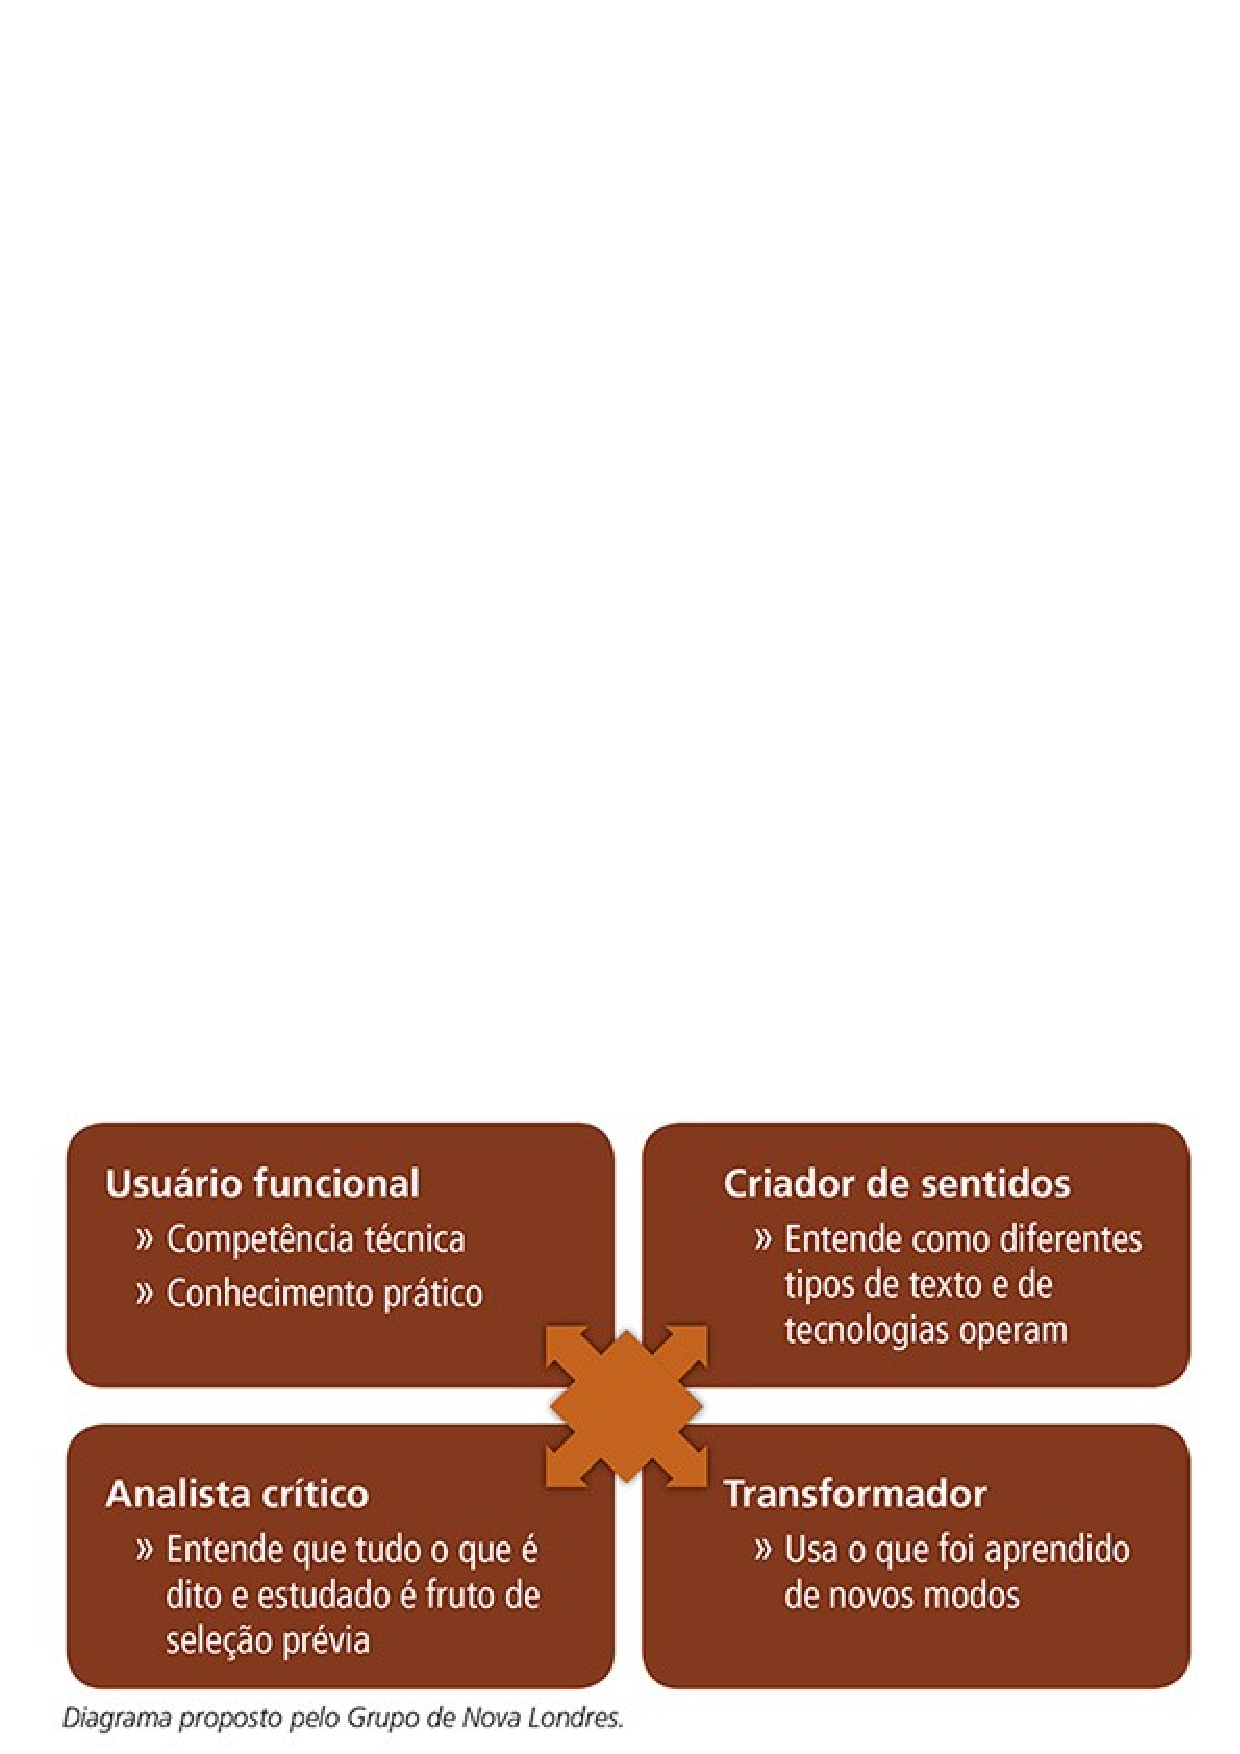
\includegraphics[width=\textwidth]{figure01.png}
\caption{Padlet criado pela equipe de enfermagem.}\label{fig-01}
\source{Arquivo pessoal.}
\end{minipage}
\end{figure}
 
Nesse caso, a professora da área pediu para que os alunos colocassem uma imagem no Padlet, criado inicialmente por ela, tendo por base a consigna “Eu cuido de mim quando…”. O intuito era trazer à discussão o repertório dos alunos acerca do cuidado do eu e do outro. A partir das imagens compartilhadas, a mediadora fez algumas perguntas aos participantes como: {\textquotedbl}\textit{Alguém do grupo pratica isso?”, “Como essas práticas relacionam-se com outras pessoas/meio ambiente?”, “Quando praticamos o que vocês trouxeram, podemos impactar o outro e o meio ambiente de alguma forma?”.}

A partir dessa etapa, os participantes “experienciaram o conhecido”, suas próprias visões do que entendiam sobre cuidado de si e do outro, ao mesmo tempo em que “experienciaram o novo”, à medida que iam visualizando/escutando o entendimento dos colegas e as considerações da professora da área de enfermagem acerca do conceito de saúde e autocuidado. Além disso, alguns deles também não conheciam a ferramenta Padlet. Na ocasião, puderam também “analisar criticamente”, quando discutiram sobre a importância do sono noturno e da prática de atividades físicas para a saúde e bem-estar, dos prejuízos causados por uma rotina de muito trabalho e de bombardeio de informações, que configuram nossa sociedade neoliberalista, do excesso de uso de telas e dos lucros que grandes empresas obtêm a partir desse consumo desenfreado da internet; além disso, discutiram o quanto esse padrão de sociedade e as nossas escolhas e estilos de vida podem equilibrar/desequilibrar o meio ambiente e o quanto isso pode contribuir ou não para o bem-estar, saúde humana e justiça social.  

No \textit{aquecimento específico}, as ações propostas buscaram o envolvimento direto dos participantes para a abordagem do tema central (neste caso, o cuidado tridimensional), preparando-os para assumir o protagonismo dentro do processo. Durante junho e julho, alunos e professores, norteados pela temática “Unidos venceremos”, desenvolveram atividades voltadas para o levantamento de questões socioambientais que impactavam/afetavam, conforme o olhar dos participantes, o “eu”, o “outro” e o “meio ambiente”. Para isso, foram realizadas atividades síncronas e assíncronas, como uma oficina virtual em que trabalhamos a análise coletiva de fotografias, o direito de imagem, o direito autoral, dicas de registro de fotografias, o aplicativo Comica e as características da técnica \textit{photovoice}, além de dois encontros síncronos por equipe, conforme a temática norteadora do mês.

Dessa forma, durante o AE, os participantes, a partir do que já conheciam e do que aprenderam no AI acerca do cuidado tridimensional, puderam “experienciar o novo” levantando as seguintes questões socioambientais: a) respeito e empatia (língua portuguesa); b) ética e ecologia (filosofia); c) consequências do desmatamento para indígenas, quilombolas e pescadores (sociologia); d) voçoroca\footnote{ Formação de grandes buracos de erosão causados pela chuva e intempéries, em solos onde a vegetação é escassa e não mais protege o solo, que fica cascalhento e suscetível de carregamento por enxurradas \cite{gomes_formacao_2021}.} (geografia); e) mapeamento socioambiental (biologia); f) saúde mental (enfermagem); g) o “eu” como agente potencial para a mudança no mundo (psicologia).

A partir do levantamento dos sete temas protagônicos citados acima, a equipe de professores aplicou um questionário para levantar a temática de maior interesse entre todos os participantes, sendo que a maioria deles optou pelo tema “saúde mental” (\Cref{fig-02}):

\begin{figure}[htbp]
\centering
\begin{minipage}{.9\textwidth}
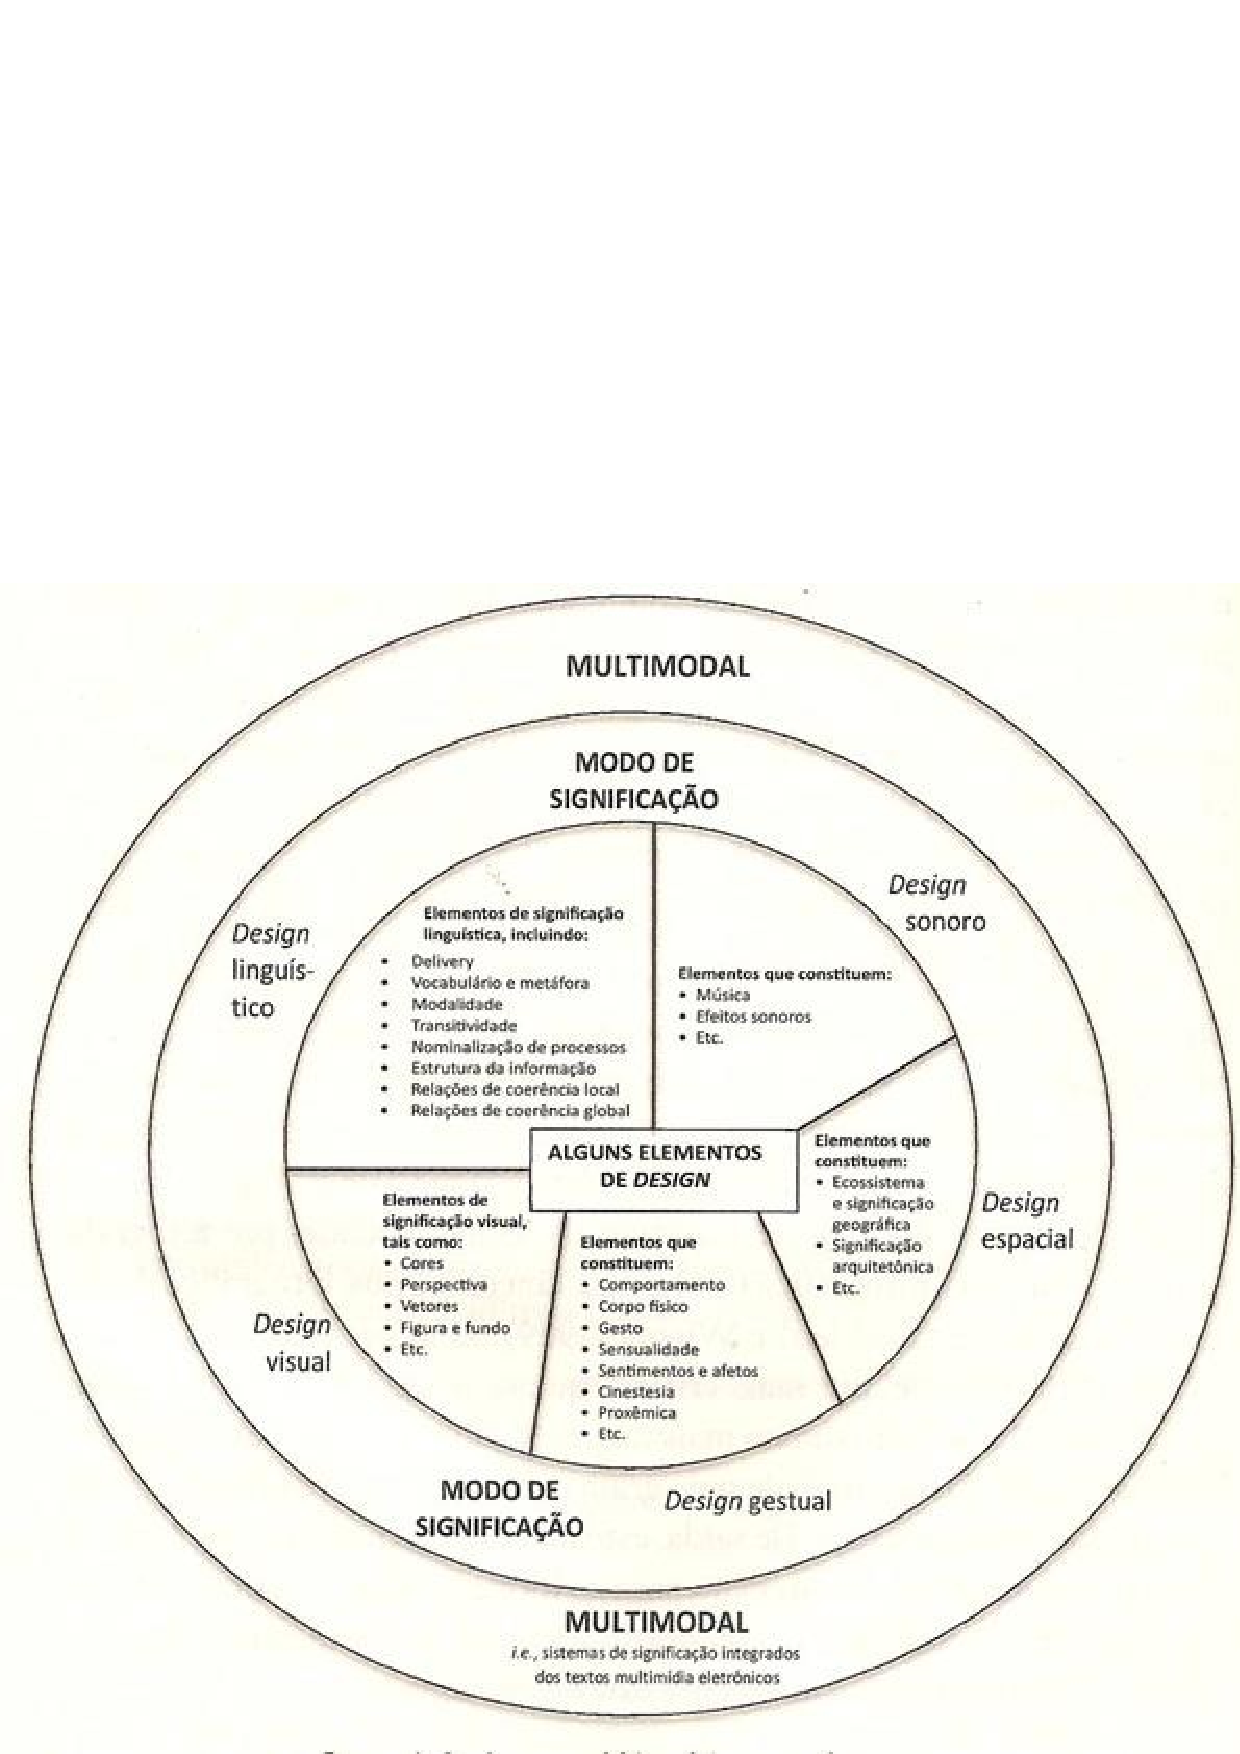
\includegraphics[width=\textwidth]{figure02.png}
\caption{Temática protagônica escolhida pelos participantes do projeto.}\label{fig-02}
\source{Arquivo pessoal.}
\end{minipage}
\end{figure}
  
Após consulta aos participantes, conforme a \Cref{fig-02}, nós professores organizamos e realizamos atividades diversificadas que atendessem, cada área à sua maneira, os temas emergidos das equipes, em especial focamos no autocuidado, nas relações respeitosas e empáticas com o(s) outro(s) e com o meio ambiente para a promoção da saúde mental e bem-estar da coletividade.

Fechamos o primeiro semestre (2021/1) realizando um encontro geral com a presença de todas as equipes e professores para compartilhamento e trocas das experiências de aprendizagem. Os participantes foram desafiados a encontrar uma forma criativa para socializar os aprendizados entre as equipes. “Aplicando criativamente” os conhecimentos adquiridos, a equipe de Língua Portuguesa lançou mão da teatralização para apresentar situações empáticas e respeitosas nas relações interpessoais como o uso de máscara e a vacinação na pandemia, abordando e refletindo os prejuízos coletivos quando não temos \textit{respeito} e \textit{empatia} nas relações sociais, em especial, no contexto pandêmico (negativismo, recusa de uso de máscaras e álcool para higienização das mãos e ambientes, queima de lixo no quintal de casa e o impacto disso para a coletividade).

Nesse contexto, a equipe de filosofia, também “aplicando criativamente”, explorou a linguagem imagética e produziu a “árvore filosofal” (\Cref{fig-03}), cheia de frutos, para compartilhar conceitos relacionados ao cuidado tridimensional. Desse modo, conforme argumentou a equipe, temos o seguinte: fruto 1 representa o planeta terra e tudo o que nele existe, o qual necessita de frutos como \textit{união} (2), \textit{colaboração} (3, 7 e 8), \textit{sabedoria} (4)\footnote{ Imagem de uma águia que representa a sabedoria, conceito discutido a partir da fábula “A águia que quase virou galinha”, de Rubem Alves, nas aulas com a equipe de filosofia.}, \textit{respeito} (5), \textit{hospitalidade e convivência} (6), \textit{acolhimento} e \textit{solidariedade} (9) e \textit{cuidado} (11 e 12). Por outro lado, o grupo “analisando criticamente” trouxe o fruto 13 simbolizando algo ruim, o não cuidado com o planeta, destacando o consumo desenfreado que resulta em grande quantidade de lixo. Os alunos encerraram o compartilhamento com a seguinte frase: “Para a ganância, toda a natureza é insuficiente” (Sêneca).  


\begin{figure}[htbp]
\centering
\begin{minipage}{.9\textwidth}
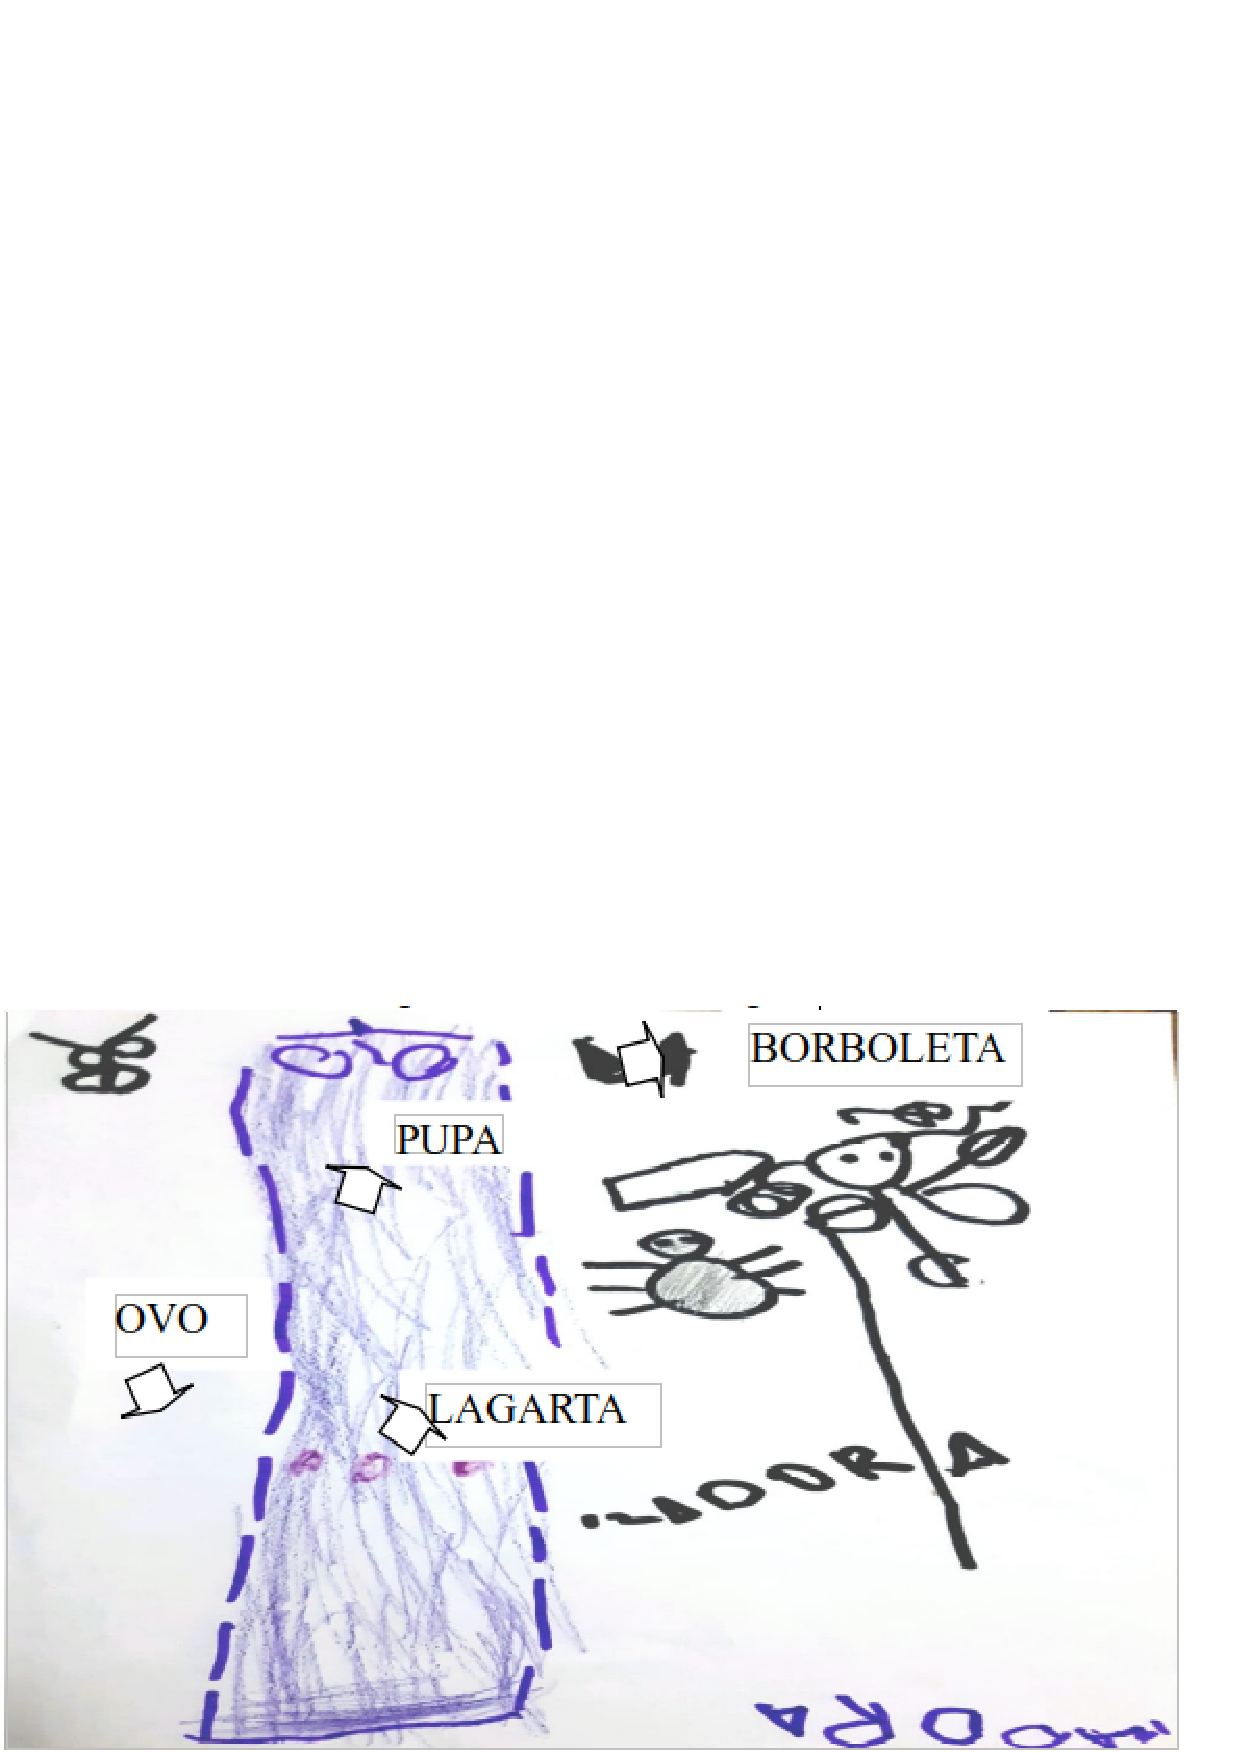
\includegraphics[width=\textwidth]{figure03.png}
\caption{A árvore filosofal produzida pela equipe de Filosofia.}\label{fig-03}
\source{Arquivo pessoal.}
\end{minipage}
\end{figure}
 

Na terceira etapa, \textit{dramatização}, momento “mão na massa”, realizada entre setembro e outubro, os estudantes, interagindo uns com outros, produziram fotografias registrando situações cotidianas que afetavam a tríade eu-outro-meio ambiente, norteados pela pergunta: \textit{Quais problemáticas socioambientais presentes em vossas realidades afetam o eu, o outro e o meio ambiente?} Nesta etapa, foi criado um mural fotográfico (\Cref{fig-04}), por meio da ferramenta Padlet, onde os estudantes iam armazenando as fotografias registradas. O mural era aberto a todos os participantes, que foram incentivados à utilização de fotografias uns dos outros, respeitando o direito autoral e dando o devido crédito ao(s) autor(es).

\begin{figure}[htbp]
\centering
\begin{minipage}{.9\textwidth}
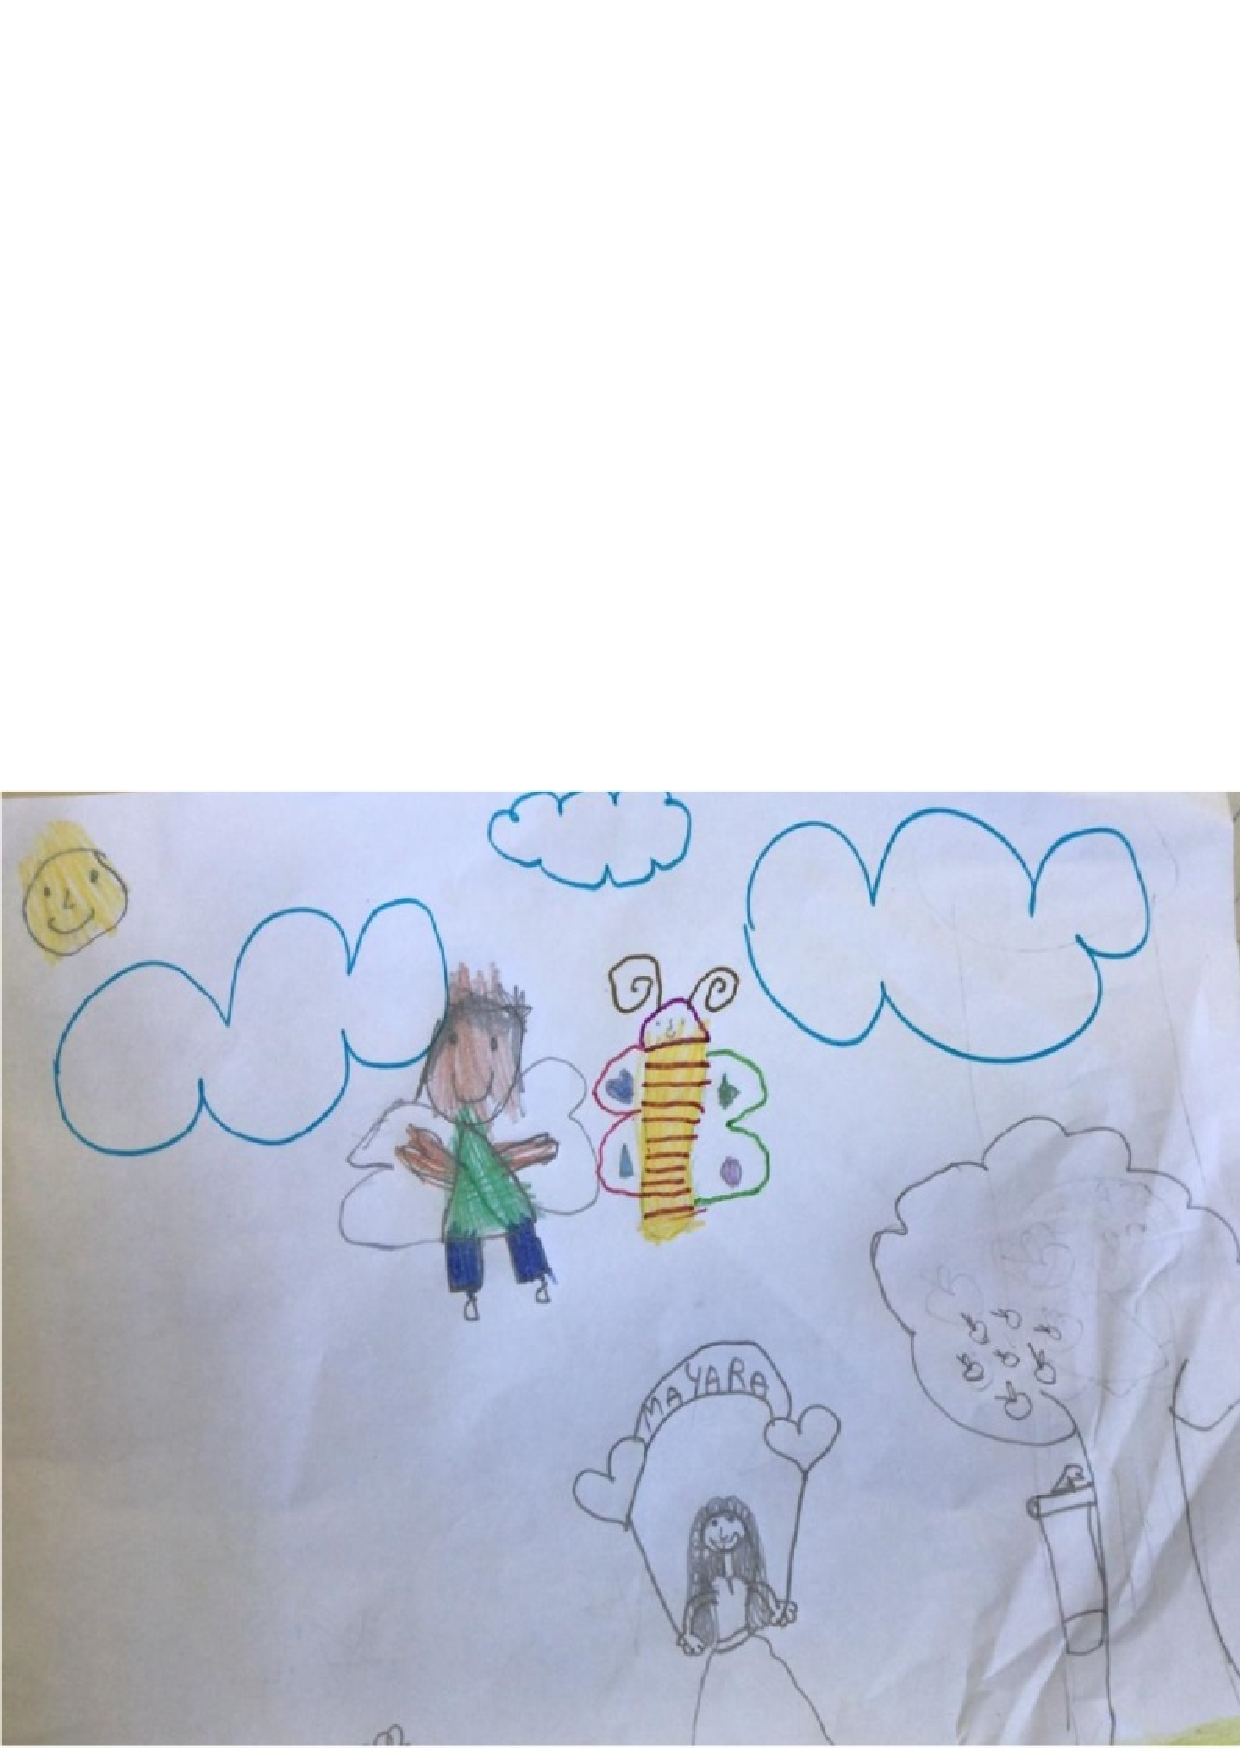
\includegraphics[width=\textwidth]{figure04.png}
\caption{Mural fotográfico do Projeto Eu, tu e o nosso ambiente.}\label{fig-04}
\source{Arquivo pessoal.}
\end{minipage}
\end{figure}
  
Para os registros fotográficos foi utilizada a técnica \textit{photovoice}, criada por \textcite{wang_photovoice:_1997}, a qual utiliza a fotografia para que as pessoas possam identificar/levantar questões importantes em suas comunidades, com o intuito de refletir e entender as suas realidades, buscando transformá-las (o que vai ao encontro da {\textquotedbl}prática transformada{\textquotedbl} prevista na teoria dos multiletramentos. As fotografias produzidas pelos participantes foram utilizadas para a construção de narrativas pessoais e em grupo/colaborativas, a partir da mixagem de linguagens verbais (escrita ou oral) e imagética. Os registros fotográficos evidenciaram dimensões tanto individual quanto colaborativa e social; além disso, serviram de base para as produções textuais multissemióticas (Histórias em Quadrinhos – HQs – e vídeos).

“Aplicando criativamente” o que aprenderam nas atividades do projeto, os participantes produziram vinte e duas Histórias em Quadrinhos, gênero textual bastante comum ao universo infanto-juvenil, as quais “por meio de seus enredos, ajudam os leitores [e autores] a ajustar suas personalidades à época e ao mundo” \cite[p. 34]{carvalho_educacao_2007}. Além disso, é um gênero que possibilita a exploração de diversos assuntos/temas; sendo assim, “analisando criticamente” os participantes exploraram as seguintes temáticas nas HQs: 

\begin{enumerate*}[label=\arabic*)]
	\item Reciclagem;
	\item preservação ambiental;
	\item desperdício de água;
	\item confiança nas relações interpessoais;
	\item importância da chuva para a vida;
	\item exclusão social;
	\item descarte inadequado de lixo;
	\item ameaça à biodiversidade;
	\item solidão;
	\item animais em situação de rua;
	\item falta de acessibilidade;
	\item queimadas;
	\item voçorocas.
\end{enumerate*}

Apropriando-se de múltiplas linguagens e recursos digitais, e a partir do olhar atento ao cotidiano motivado pelos professores das áreas envolvidas no projeto, os alunos produziram sentidos por meio de textos autorais e criativos. Para \textcite[p. 307]{santos_letramento_2011}, a produção das HQs não pressupõe apenas “juntar palavras e imagens, antes, relacioná-las” no processo de produção de sentido.

A etapa final do projeto foi reservada ao \textit{compartilhamento }(novembro e dezembro)\textit{, }momento em que os participantes, “aplicando criativamente”, socializaram o conhecimento em eventos institucionais como a Semana de Ciência e Tecnologia (roda de conversa entre professores e alunos) e o Festival de Arte e Cultura (apresentação de vídeos) do IFMS. Além disso, ainda “analisando criticamente”, fizemos um encontro síncrono \textit{on-line} com músicas selecionadas pelos participantes cujas letras relacionavam-se com o cuidado tridimensional; “teia” de agradecimentos afetuosa entre os participantes; jogos em grupos que abordaram assuntos relacionados ao projeto, além da apresentação de uma paródia da música \textit{Será}\footnote{ Para acesso à paródia, acesse: \url{https://drive.google.com/file/d/166ss42qra_vChO5tjLIKRmCSbi_G13b6/view?usp=sharing}.}, do grupo Legião Urbana, em que a equipe da geografia abordou e analisou criticamente o problema das voçorocas que afetam a cidade de Nova Andradina e a região do vale do Ivinhema, no Mato Grosso do Sul.

É importante ressaltar que os quatro processos do conhecimento não são lineares. Cada prática pedagógica tem um propósito e a depender disso é que os envolvidos no processo vão explorando-os de acordo com os objetivos de aprendizagem e os resultados pretendidos, conforme notamos em nosso projeto e buscamos ilustrar aqui.

\section{Formação crítica: criatividade, colaboração e agência}\label{sec-formaçãocrítica-criatividade}

Quando pensamos no uso de tecnologias digitais na educação, caminhamos por uma linha tênue do neoliberalismo, na qual, é desafiador saber onde termina o educacional e começa o mercadológico \cite{ball_nova_2014}, pois a lógica neoliberal é que as duas instâncias caminham juntas. Como propõe \textcite{buzato_inteligencia_2023}, o propósito é uma análise crítica das relações entre o humano e o digital para que não caiamos nos jogos das relações mercadológicas de tecnologias digitais. Destacamos, ainda, que as mídias digitais por si só não são capazes de promover uma formação crítica e criativa, mas sim as ações, a criatividade, a sensibilidade dos professores e alunos envolvidos no processo que fazem a diferença.

Foi nesse sentido que a prática relatada no presente artigo buscou um esforço de atuação dentro de um novo \textit{ethos} \cite{knobel_new_2007}, na tentativa de contribuir para a formação de um sujeito crítico, participativo e criativo, dentro de práticas situadas, interdisciplinares e colaborativas conectadas à realidade a que pertence: digital e pandêmica.

A formação desse sujeito crítico a qual nos referimos incide sobretudo sobre  a agência do aluno, ligada à capacidade de avaliar e agir frente ao que foge do esperado \cite[p. 1]{monte_mor_development_2013}, a partir do desenvolvimento de consciência crítica social. É nesse sentido que buscamos uma prática situada ao contexto dos alunos e dos professores frente ao ciberespaço e a sociedade em rede na pandemia da Covid-19; conceitualizar com teoria a partir de pesquisa e trabalho teórico do projeto; analisar criticamente a realidade vivenciada a partir das atividades listadas ao longo da nossa discussão; além da prática transformada, aplicada criativamente por meio de vídeos e HQs divulgados à comunidade.

Pensando nas atividades desenvolvidas, é pertinente destacar a relação de um novo \textit{ethos} \cite{knobel_new_2007} ao prefixo “multi” de multiletramentos. \textcite{knobel_new_2007} consideram que as novas tecnologias proporcionam uma nova ordem social e não simplesmente atualizam as ferramentas já utilizadas. Tal posicionamento também serve aos multiletramentos que não tratam somente da construção de sentido por meio de tecnologias digitais, mas pela multiplicidade semiótica. Por isso, \textcite{duboc_delinking_2021} sugerem o {\textquotedbl}desprendimento{\textquotedbl}\footnote{ No original: \textit{delinking}.} dos multiletramentos à ligação fixa ao digital.

Essa discussão é pertinente, pois é por meio dos registros fotográficos que os alunos são sensibilizados e se deparam com a amplitude da problemática trabalhada no projeto, ou seja, não se trata somente de uma reconfiguração de aprendizagem a partir de tecnologias digitais, mas, sim, como o \textit{ethos} do aluno foi redesenhado para que a construção de sentido acontecesse, o que se deu a partir de um contexto amplo de caracteres do ciberespaço e da sociedade em rede.


	Na prática relatada e discutida neste trabalho, vemos um aluno sensibilizado pelos problemas sociais da sua cidade, do seu entorno, em um período pandêmico e de aulas remotas. Os próprios alunos destacam no projeto as relações entre as atividades propostas e questões sociais – por vezes do seu entorno –, não o uso de tecnologias digitais por si só.


	A nosso ver, o diferencial não está na tecnologia digital por si só, mas nas relações estabelecidas entre os sujeitos e as ferramentas digitais, dentro de um contexto amplo de multiletramentos, no qual ações colaborativas e criativas podem resultar em práticas significativas para o bem-estar da coletividade.


	Vemos também a agência do professor no projeto, ao considerar o contexto dos alunos, a diversidade das formas de aprender por meio dos diversos recursos utilizados, a mediação por questionamentos e a divulgação e reconhecimento dos trabalhos finais para a comunidade.

No caminho do projeto (experienciar o novo; conceitualizar com teoria; aplicar criativamente; e analisar criticamente.), conseguimos olhar para as relações entre humano/digital, múltiplas e hibridizadas, de forma crítica e por meio da agência do professor e do aluno, significativas às agendas não neoliberais de educação e tecnologias digitais.
\section{Considerações finais}\label{sec-consideraçõesfinais}

A partir da análise da vivência educacional descrita, visualizamos as interações propiciadas pelo novo \textit{ethos}, advindo do ciberespaço e da cultura digital, em especial, em contexto pandêmico, no qual as múltiplas semioses foram articuladas e propiciaram o exercício de consciência e agência dos alunos e dos professores.

Os participantes puderam olhar criticamente para as relações entre o eu, o outro e o meio ambiente em suas comunidades locais, problematizando questões socioambientais durante a pesquisa e o registro fotográfico, além de agir socialmente mediante a produção de vídeos e HQs que foram divulgados à comunidade em geral em eventos institucionais, bem como na internet.

Além disso, a técnica \textit{photovoice} aliada aos multiletramentos e à pedagogia psicodramática potencializou a mixagem de gêneros, mídias e linguagens, cara ao novo \textit{ethos} proveniente da cultura digital, na qual fontes, autorias e gêneros se articulam de forma rizomática.

Reconhecidos os limites deste texto e de todo trabalho educacional – que se estabelece na tênue linha educação-mercado –, esperamos que ele possa ajudar a pensar em alguns caminhos para o trabalho crítico com tecnologias digitais em sala de aula, de forma colaborativa e interdisciplinar e com foco em questões de linguagem.



\printbibliography\label{sec-bib}
%full list: conceptualization,datacuration,formalanalysis,funding,investigation,methodology,projadm,resources,software,supervision,validation,visualization,writing,review
\begin{contributors}[sec-contributors]
\authorcontribution{Luciene Bomfim}[conceptualization,datacuration,investigation,methodology,projadm,writing,review]
\authorcontribution{Fabiana Biondo}[conceptualization,methodology,supervision,writing,review]
\authorcontribution{Iasmin Maia}[conceptualization,methodology,writing,review]
\end{contributors}

\end{document}
